% !TeX spellcheck = pt_BR
% !TeX encoding = UTF-8
% Escolha: portugues ou ingles ou espanhol.
% Para a versão final do texto, após a defesa acrescente final:

% Para o exame de qualificação
%\documentclass[portugues, qualificacao]{ic-tese}
% Para a tese
\documentclass[portugues]{ic-tese}
% Para a versão final da tese
%\documentclass[portugues,final]{ic-tese}

% Extra macros para escrita 
%\usepackage{ic-extras}

\usepackage[latin1,utf8]{inputenc}
\usepackage{pifont}

%% Math
\usepackage{mathtools}
\usepackage{amsmath}
\usepackage{commath}

\usepackage{amsfonts}% revise se precisa ou não
\usepackage{nccmath}% revise se precisa ou não

\usepackage[numbers]{natbib}

\newcommand\citetxt[1]{%
  \citeauthor{#1}~(\citeyear{#1})}
\newcommand\citepar[1]{%
  (\citeauthor{#1}, \citeyear{#1})} 


%% tight space around equations
%\apptocmd\normalsize{%
%  \abovedisplayskip=7pt plus 2pt minus 7pt
%  \abovedisplayshortskip=0pt plus 3pt
%  \belowdisplayskip=7pt plus 2pt minus 6pt
%  \belowdisplayshortskip=4pt plus 3pt minus 4pt
%}{}{}
%
%\abovedisplayskip=0pt
%\belowdisplayskip=0pt

\newcommand{\conc}{\mathbin{\Vert}}

% Adaptive norm operator
% https://tex.stackexchange.com/a/70130/7561
% With this setup, \norm*{...} will produce automatically sized double-bar
% fence symbols around the macro's, whereas (say) \norm[\bigg]{...} will
% generate \bigg double-bar symbols. There are four sizing modifiers: \big,
% \Big, \bigg, and \Bigg. 

%https://tex.stackexchange.com/q/151984/7561
\DeclarePairedDelimiterX{\infdivx}[2]{(}{)}{%
  #1\;\delimsize\|\;#2%
}
\newcommand{\kl}{\operatorname{KL}\infdivx}
\newcommand{\skl}{\operatorname{SKL}\infdivx}

% https://tex.stackexchange.com/questions/23773/a-centered-plus-minus-symbol
\newcommand{\rpm}{\raisebox{.2ex}{$\scriptstyle\pm$}}

% https://tex.stackexchange.com/a/141685/7561
\newcommand\givenbase[1][]{\:#1\lvert\:}
\let\given\givenbase

% https://tex.stackexchange.com/a/171959/7561
\newcommand\reallywidehat[1]{\ThisStyle{%
    \setbox0=\hbox{$\SavedStyle#1$}%
    \stackengine{-1.0\ht0+.5pt}{$\SavedStyle#1$}{%
      \stretchto{\scaleto{\SavedStyle\mkern.15mu\char'136}{1.5\wd0}}{1.4\ht0}%
    }{O}{c}{F}{T}{S}%
}}
\newcommand{\hkl}{\widehat{\operatorname{KL}}\infdivx}

% Conditional independence symbol
% https://tex.stackexchange.com/questions/218631/symbol-for-not-conditionally-independent/
\newcommand{\CI}{\mathrel{\perp\mspace{-10mu}\perp}}

% declare my argmin and argmax operators
% https://tex.stackexchange.com/a/5255/7561
\DeclareMathOperator*{\argmax}{arg\,max}
\DeclareMathOperator*{\argmin}{arg\,min}

% declaring an expectation operator to behave like sum
% https://tex.stackexchange.com/a/23436/7561
\makeatletter
\DeclareRobustCommand\bigop[1]{%
  \mathop{\vphantom{\sum}\mathpalette\bigop@{#1}}\slimits@
}
\newcommand{\bigop@}[2]{%
  \vcenter{%
    \sbox\z@{$#1\sum$}%
    \hbox{\resizebox{\ifx#1\displaystyle.9\fi\dimexpr\ht\z@+\dp\z@}{!}{$\m@th#2$}}%
  }%
}
\makeatother

%\newcommand{\E}{\DOTSB\bigop{\mathbb{E}}}
\DeclareMathOperator*{\E}{\mathbb{E}}

% redefining \times operator
\let\oldtimes\times
\def\times{{\mkern1mu\oldtimes\mkern1mu}}



\usepackage{subfigure}
\newcommand{\cmark}{\ding{51}}%

%\DeclarePairedDelimiter\abs{\lvert}{\rvert}%
%\DeclarePairedDelimiter\norm{\lVert}{\rVert}%
\DeclarePairedDelimiter\product{\langle}{\rangle}%

\usepackage{cellspace}
\setlength\cellspacetoplimit{6pt}
\setlength\cellspacebottomlimit{4pt}

%% Units
\usepackage{siunitx}

%% Tables
\usepackage{booktabs}


% Para acrescentar comentários ao PDF descomente:
\usepackage
%  [pdfauthor={nome do autor},
%   pdftitle={titulo},
%   pdfkeywords={palavra-chave, palavra-chave},
%   pdfproducer={Latex with hyperref},
%   pdfcreator={pdflatex}]
{hyperref}

% Os cores podem ser mudados
\hypersetup{
%  linkcolor={red!50!black},
%  citecolor={blue!50!black},
%  urlcolor={blue!80!black}
}

\begin{document}

% Escolha entre autor ou autora:
\autor{Thales Eduardo Nazatto}
%\autora{Nome da Autora}

% Sempre deve haver um título em português:
\titulo{Construção de um \textit{Pipeline} de \textit{Machine Learning} autônomo com métricas de \textit{Fairness}}
\title{text}

% Se a língua for o inglês ou o espanhol defina:
%\title{The Dissertation or Thesis Title in English or Spanish}

% Escolha entre orientador ou orientadora. Inclua os títulos acadêmicos:
%\orientador{Prof. Dr. Gerberth Adín Ramírez Rivera}
\orientadora{Profa. Dra. Cecília Mary Fischer Rubira}

% Escolha entre coorientador ou coorientadora, se houver.  Inclua os títulos acadêmicos:
\coorientador{Prof. Dr. Leonardo Montecchi}
%\coorientadora{Prof. Dra. Eng. Lic. Nome da Co-Orientadora}

% Escolha entre mestrado ou doutorado:
\mestrado
%\doutorado

% Se houve cotutela, defina:
%\cotutela{Universidade Nova de Plutão}

\datadadefesa{30}{07}{2022}

% Para a versão final defina:
%\avaliadorA{Prof. Dr. Primeiro Avaliador}{Instituição do primeiro avaliador}
%\avaliadorB{Profa. Dra. Segunda Avaliadora}{Instituição da segunda avaliadora}
%\avaliadorC{Dr. Terceiro Avaliador}{Instituição do terceiro avaliador}
%\avaliadorD{Prof. Dr. Quarto Avaliador}{Instituição do quarto avaliador}
%\avaliadorE{Prof. Dr. Quinto Avaliador}{Instituição do quinto avaliador}
%\avaliadorF{Prof. Dr. Sexto Avaliador}{Instituição do sexto avaliador}
%\avaliadorG{Prof. Dr. Sétimo Avaliador}{Instituição do sétimo avaliador}
%\avaliadorH{Prof. Dr. Oitavo Avaliador}{Instituição do oitavo avaliador}


% Para incluir a ficha catalográfica em PDF na versão final, descomente e ajuste:
%\fichacatalografica{arquivo.pdf}


% Este comando deve ficar aqui:
\frontmatter


% Se houver dedicatória, descomente:
%\prefacesection{Dedicatória}
%A dedicatória deve ocupar uma única página.


% Se houver epígrafe, descomente e edite:
% \begin{epigrafe}
% {\it
% Vita brevis,\\
% ars longa,\\
% occasio praeceps,\\
% experimentum periculosum,\\
% iudicium difficile.}
%
% \hfill (Hippocrates)
% \end{epigrafe}


% Agradecimentos ou Acknowledgements ou Agradecimientos
%\chapter{Agradecimentos}
%Os agradecimentos devem ocupar uma única página.


% Sempre deve haver um resumo em português:
\begin{resumo}
Esta dissertação de Mestrado possui o objetivo de contribuir com o tema de Inteligência Artificial (IA) do ponto de vista da Engenharia de Software, visto que o uso de IA envolvendo grandes volumes de dados vem crescendo conforme nossa sociedade migra processos manuais de trabalho para soluções digitais e necessita de tomadas de decisão mais rápidas e assertivas. Entretanto, as métricas usadas inicialmente para definir a eficácia de um algoritmo se mostraram limitadas devido a barreiras éticas e legais, resultando em vieses que refletem a sociedade de maneira que não era esperada pelos desenvolvedores da solução. Desta forma, o uso de novas métricas, como métricas de Fairness, e proveniência de dados pode ajudar neste problema. Desenvolvendo um pipeline autônomo utilizando a arquitetura MAPE-K, documentando métodos e ferramentas, e realizando estudos de caso, é esperado que este problema seja controlado e facilite o desenvolvimento de softwares com o uso responsável de dados.
\end{resumo}


% Sempre deve haver um abstract:
\begin{abstract}
This Master's Degree dissertation aims to contribute to the theme of Artificial Intelligence (AI) from the Software Engineering point of view, since the use of AI involving large volumes of data has been growing as our society migrates manual work processes to digital solutions and needs faster and more assertive decision making. However, the metrics used initially to define the effectiveness of an algorithm proved to be limited due to ethical and legal barriers, resulting in biases that reflect society in a way that was not expected by the solution developers. Thus, the use of new metrics, like Fairness metrics, and data provenance can help with this problem. By developing an autonomous pipeline using MAPE-K architecture, documenting methods and tools, and making case studies, it is expected that this problem will be controlled and facilitate software development with the responsible use of data.
\end{abstract}


% Se houver um resumo em espanhol, descomente:
%\begin{resumen}
% A mesma regra aplica-se.
%\end{resumen}


% A lista de figuras é opcional:
% \listoffigures

% A lista de tabelas é opcional:
% \listoftables

% A lista de abreviações e siglas é opcional:
% \prefacesection{Lista de Abreviações e Siglas}

% A lista de símbolos é opcional:
% \prefacesection{Lista de Símbolos}

% Quem usa o pacote nomencl pode incluir:
%\renewcommand{\nomname}{Lista de Abreviações e Siglas}
%\printnomenclature[3cm]


% O sumário vem aqui:
\tableofcontents


% E esta linha deve ficar bem aqui:
\mainmatter

%\mainmatter

\chapter{Introdução}

% O corpo da dissertação ou tese começa aqui:
Técnicas de Inteligência Artificial e Aprendizado de Máquina já são utilizadas há bastante tempo no ramo da Computação. Ramos como robótica e jogos são grandes exemplos, dada a necessidade nos mesmos de automatizar comportamentos que seriam tidos como triviais para um ser humano. Entretanto, nos últimos anos ocorreu um crescimento no uso dessas tecnologias em aplicações tradicionais, com previsão de US\$ 57 bilhões em investimentos em 2021, 480\% maior em relação a 2017~\citep{Deloitte_2018}. No Brasil, o número de empresas de IA aumentou de 120 em 2018 para 206 em 2020~\citep{CIO_2021}.

Isso se mostra possível devido a grande quantidade de dados processada diariamente pelas empresas, que coletam estatísticas toda vez que um usuário acessa suas aplicações. Com esses dados, podem traçar diferentes perfis e usar soluções de IA para ter tomadas de decisão mais assertivas com o objetivo de melhorar a experiência de usuário e corrigir problemas. Porém, muitas dessas soluções foram projetadas sem pensar em governança de dados como requisito de projeto, e se mostram ineficientes quando ela é tratada em consideração.

Governança de dados é um tema que entrou em evidência recentemente em países como o Brasil: Iniciativas como a LGPD - Lei Geral de Proteção de Dados \citep{LGPD_2021}, de 14 de agosto de 2018, mostram como as aplicações e seus dados possuem cada vez mais influência na sociedade moderna. E nesse ponto muitas aplicações de IA falham: muitas implementações foram implementadas como \textit{black boxes}, onde o determinante para estabelecer a confiança no modelo implementado é sua entrada e sua saída.

Um outro efeito colateral dessa estratégia é a exposição de vieses que, embora sejam vistos como não-intencionais pelos desenvolvedores por ter a possibilidade de ser um \textit{outlier} no modelo treinado, refletem preconceitos escancarados da sociedade atual. Uma entrada de dados enviesada resulta em um algoritmo que realiza discriminações em sua classificação~\citep{Buolamwini_2018}, e uma vez que as métricas utilizadas para medir a qualidade de um modelo \textit{black box} são geralmente baseadas em acurácia, precisão e recall, discriminações não são facilmente percebidas por tais métricas. Ao mesmo tempo, um modelo \textit{black box} pode ter uma alta dependência de poucos dados, determinando problemas de acoplamento. Para resolver este problema, é possível que a criação de um novo modelo seja uma melhor opção que realizar a correção em apenas parte dele.

Devido a esses tipos de problemas, o termo \textit{Explainable AI} (XAI) ganha força para envolver o desenvolvimento de uma IA que seja acurada e simultaneamente transparente. Como IA possui diversos tipos de métodos diferentes para enquadrar diversos tipos de dados, o mesmo acaba se aplicando em Explainable AI, podendo enquadrar em diversos tipos de dados~\citep{Sundararajan_2017}, ou dados específicos como imagens~\citep{Kapishnikov_2019} e tabelas~\citep{Maleki_2013}. Como o objetivo em XAI é fazer com que os resultados alcançados pela solução de IA sejam compreendidos por humanos, é possível considerar este fato como requisito no design de uma solução de IA, fazendo com que a mesma seja reusável e testável.

No mesmo tema, é possível estabelecer métricas para determinar o quão o modelo está preparado para dados sensíveis \citep{Begley_2021}, termo que é conhecido como \textit{Fairness}. Com a evolução das pesquisas na comunidade acadêmica, foram descobertos algoritmos para redução dos vieses presentes nos conjuntos de dados, como \textit{Reweighing}~\citep{Kamiran_2011}, \textit{Adversarial Debiasing}~\citep{Zhang_2018} e \textit{Reject Option Classification}~\citep{Kamiran_2012}. Por consequência, ocorre melhora nas métricas em questão, mas pode desfavorecer métricas que já são amplamente utilizadas como garantia de um bom modelo desenvolvido com técnicas de Aprendizado de Máquina.

O objetivo desta dissertação de mestrado é desenvolver uma estrutura de \textit{Pipeline} para \textit{Machine Learning} que seja completamente autônoma, por três fatores principais:

\begin{itemize}
\item Facilitar a criação de modelos justos e confiáveis com a automatização da escolha dos algoritmos, cuja complexidade aumenta com a escolha dos algoritmos a serem utilizados e suas execuções nas etapas corretas do processo, onde eles foram escolhidos para atuar.
\item Estabelecer um balanceamento entre métricas para avaliar bons modelos com métricas para avaliar modelos justos.
\item Considerar proveniência de dados como requisito no design de uma solução de IA, e como uma alternativa a XAI através da utilização de metadados.
\end{itemize}

Para isso, além do desenvolvimento do \textit{Pipeline} em questão, será utilizada a arquitetura MAPE-K~\citep{IBM_2005} para analisar uma base de conhecimento e prover o melhor pipeline seguindo regras pré-determinadas.

O restante da dissertação se organizará da seguinte forma: o Capítulo 2 descreve os conceitos que irão ser abordados neste projeto; o Capítulo 3 mostra a metodologia e detalhamento do processo de desenvolvimento; o Capítulo 4 discute os resultados obtidos e, finalmente, o Capítulo 5 estabelece as conclusões, considerações finais e sugestões de trabalhos futuros e evoluções.

\chapter{Conceitos Relacionados}

\section{Ciência de Dados e Engenharia de Dados}

\section{Machine Learning}

Aprendizado de Máquina (\textit{Machine Learning}, em inglês) pode ser definido como “a prática de usar algoritmos para coletar dados, aprender com eles, e então fazer uma determinação ou predição sobre alguma coisa no mundo. Então em vez de implementar as rotinas de software manualmente, com um gama específica de instruções para completar uma tarefa em particular, a máquina é `treinada` usando uma quantidade grande de dados e algoritmos que dão e ela a habilidade de aprender como executar a tarefa”~\citep{Copeland_2016}. Com isso, o computador consegue a habilidade de realizar determinado cálculo ou tarefa sem que necessite de programação adicional ou interferência humana para isso.

O \textit{Machine Learning} é fortemente relacionado com a Estatística, uma vez que seus métodos e parte de seus algoritmos, como regressões, tiveram como base modelos estatísticos e a análise de seus dados. As tarefas de aprendizado podem ser classificadas em três categorias básicas~\citep{MLWikipedia_2021}~\citep{MLSAS_2021}:

\begin{itemize}
\item \textbf{Aprendizado supervisionado}: O treinamento é realizado por meio de exemplos rotulados, como uma entrada na qual a saída desejada é conhecida. Através de métodos como classificação, regressão e \textit{gradient boosting}, o aprendizado supervisionado utiliza padrões para prever os valores de rótulos em dados não-rotulados adicionais. O aprendizado supervisionado é comumente empregado em aplicações nas quais dados históricos preveem eventos futuros prováveis.
\item \textbf{Aprendizado não-supervisionado}: É utilizado em dados que não possuem rótulos históricos. A “resposta certa” não é informada ao sistema, o algoritmo deve descobrir o que está sendo mostrado. O objetivo é explorar os dados e encontrar alguma estrutura dentro deles. Técnicas populares incluem mapas auto-organizáveis, mapeamento por proximidade, agrupamento \textit{k-means} e decomposição em valores singulares. Esses algoritmos também são utilizados para segmentar tópicos de texto, recomendar itens e identificar pontos discrepantes nos dados.
\item \textbf{Aprendizado por reforço}: O algoritmo descobre através de testes do tipo “tentativa e erro” quais ações rendem as maiores recompensas. Este tipo de aprendizado possui três componentes principais: o agente (o aprendiz ou tomador de decisão), o ambiente (tudo com que o agente interage) e ações (o que o agente pode fazer). O objetivo é que o agente escolha ações que maximizem a recompensa esperada em um período de tempo determinado. O agente atingirá o objetivo muito mais rápido se seguir uma boa política, então o foco do aprendizado por reforço é descobrir a melhor política.
\end{itemize}

O termo \textit{Machine Learning} se tornou muito mais evidente com a possibilidade da implementação do \textit{Deep Learning}, que é uma técnica que utiliza Redes Neurais Artificiais para atingir seus resultados. Redes Neurais Artificiais são modelos computacionais inspirados no sistema nervoso do cérebro, onde temos neurônios divididos em camadas e conectados entre si, podendo ser abstraído conforme ilustração na Figura \ref{fig:NeuralNetwork}. Dependendo da tarefa a ser realizada, cada neurônio atribui um peso para os dados que entram e a saída final é determinada pelo total desses pesos~\citep{Copeland_2016}. As redes neurais utilizadas em \textit{Deep Learning} possuem, ao menos, duas camadas de neurônios entre a camada que recebe os dados de entrada e a camada final que faz o tratamento final dos dados de saída.

\begin{figure}[h]
\centering
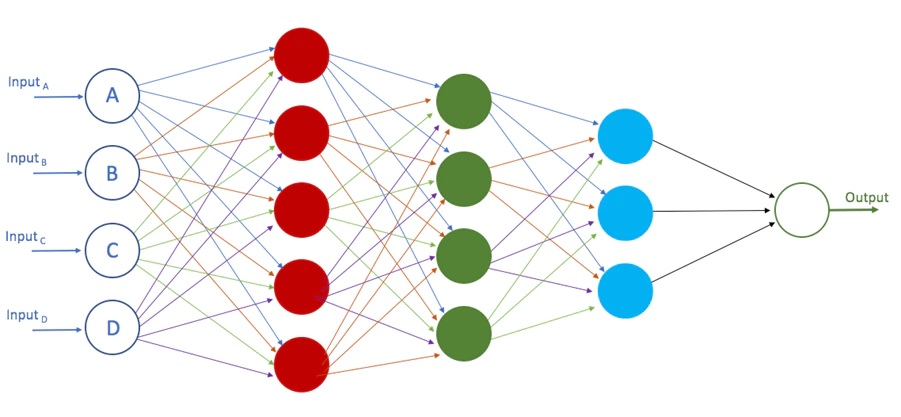
\includegraphics[scale=0.8]{images/deep_neural_network.jpg}
\caption {Exemplo de uma rede neural utilizada em \textit{Deep Learning}.}
\label{fig:NeuralNetwork}
\end{figure}

Com a evolução da computação, o treino de uma tarefa passou a ser cada vez mais viável, uma vez que a execução de algoritmos de \textit{Machine Learning} é computacionalmente muito custosa, especialmente quando redes neurais são utilizadas. E sua viabilidade é acompanhada de efetividade: Como exemplo, reconhecimento de imagens por máquinas treinadas através de deep learning em alguns cenários possuem uma taxa de acerto maior que a de humanos~\citep{Copeland_2016}.

\subsection{Métricas de Avaliação}

\subsection{Algoritmos}

\section{Fairness em Machine Learning}

\subsection{Métricas de Fairness}

\section{Algoritmos para redução de vieses}

\section{AI Explainability}

\textit{AI Explainability} é um conceito em IA que propõe a criação de um conjunto de técnicas de Aprendizado de Máquina (ou Machine Learning/ML) que produz modelos mais explicáveis, mantendo qualidade em suas métricas, e permite que os humanos entendam, confiem e gerenciem aplicações baseadas em IA. XAI também absorve conceitos das Ciências Sociais e considera a psicologia da explicação~\citep{Arrieta_2020}. Um algoritmo de ML explicável precisa não apenas mostrar tomadas de decisão, mas também mostrar o processo que o levou ao tomar tal decisão, de modo que seja compreensível e transparente para humanos.

\begin{figure}[h]
\centering
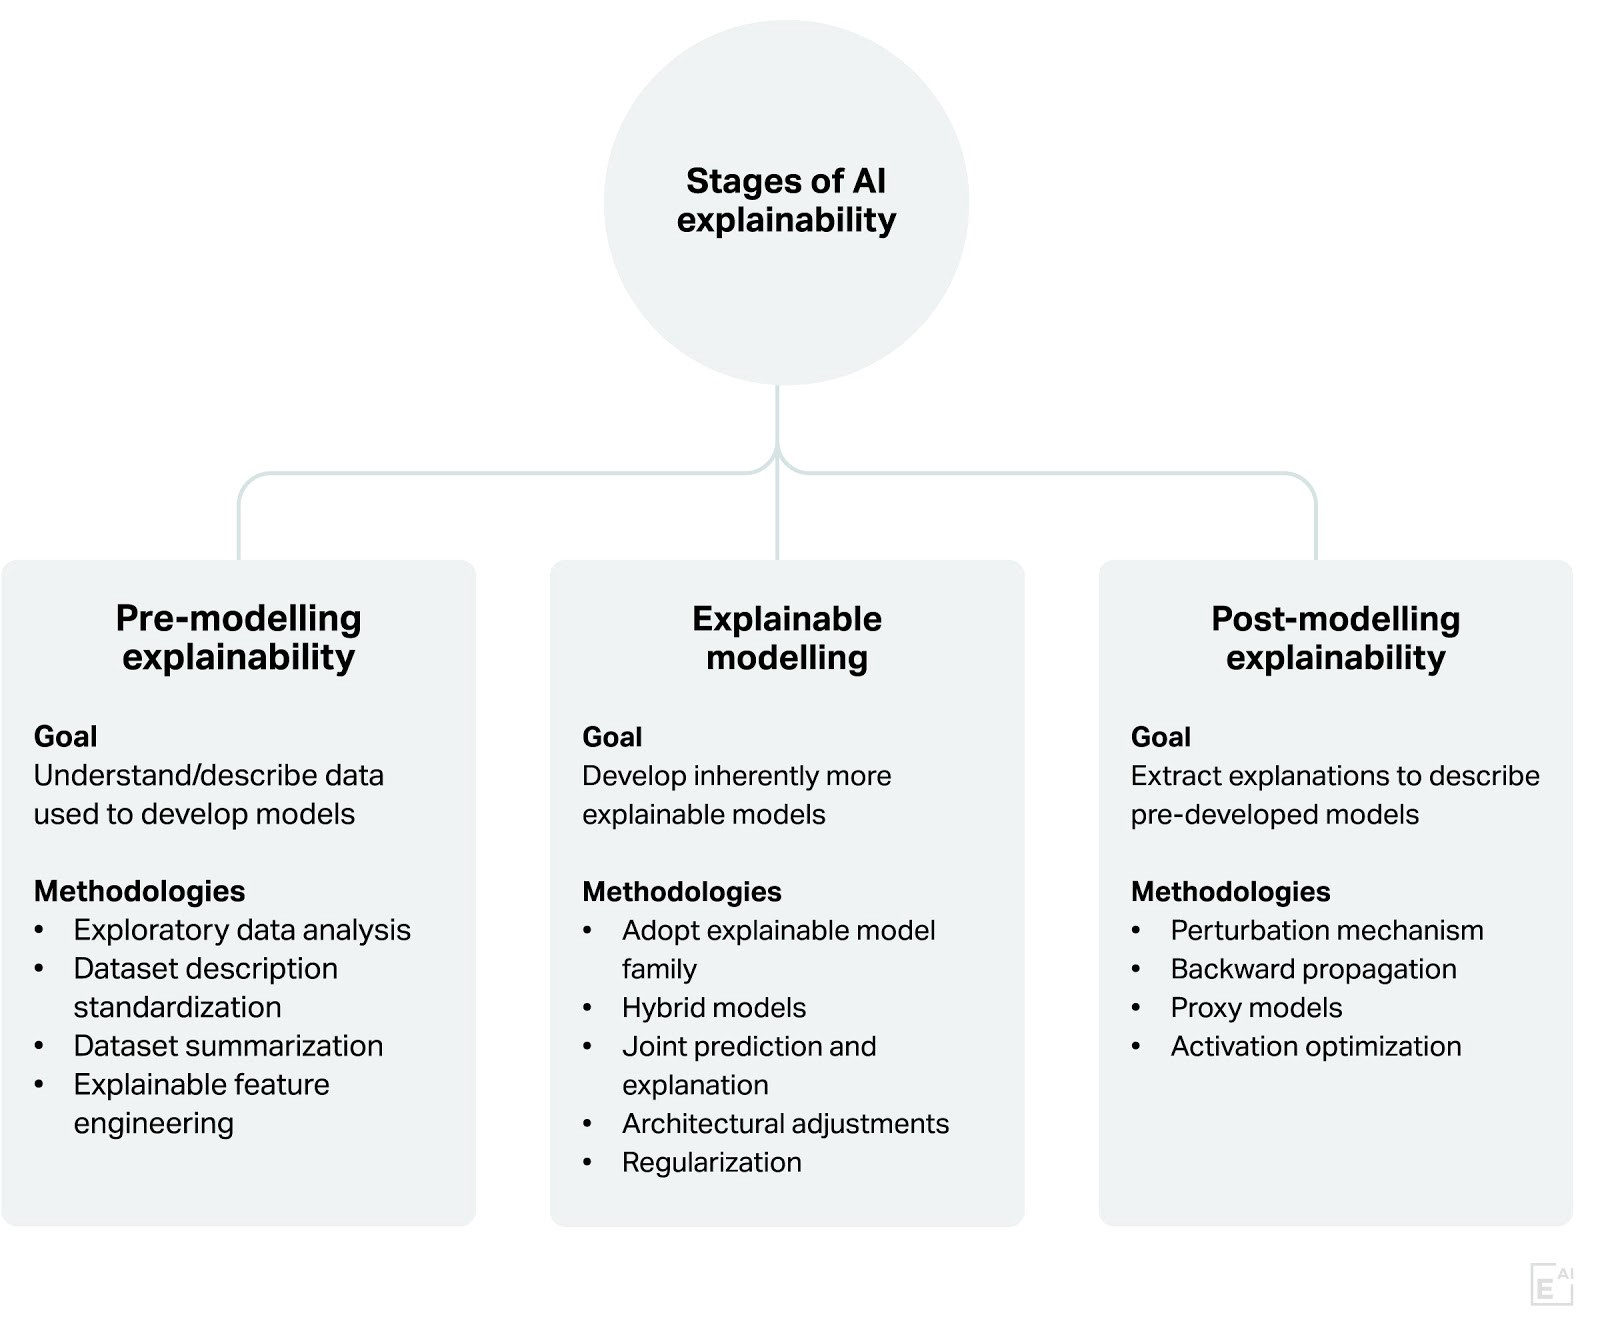
\includegraphics[scale=0.2]{images/phases.jpeg}
\caption {Fases de um processo baseado em IA explicável.}
\label{fig:StagesExplainableAI}
\end{figure}

Conforme ilustrado na Figura \ref{fig:StagesExplainableAI}, o um processo baseado em IA explicável pode ser classificado em 3 fases:

\begin{itemize}
\item \textbf{\textit{Pre-Modelling Explainability}:} Esta fase se caracteriza por obter explicações no conjunto de dados usado para treino e validação, tendo como principal motivação o fato do comportamento de um modelo depender muito dos dados que o alimentam. Análises e visualizações dos dados, ou mesmo através de documentações do conjunto de dados se enquadram neste estágio.~\citep{Khalegi_2019_Pre} 
\item \textbf{\textit{Explainable Modelling}:} Esta fase se caracteriza por obter explicações por modelos considerados transparentes (ver adiante). Ao adotar modelos deste tipo, ele já pode ser considerado como explicável por um humano. Também é possível obter a explicação através de regularizadores, ou adotar abordagens onde explicação e resultado sejam obtidos simultaneamente, sejam via junção de dados ou sendo intrínseco a arquitetura do modelo.~\citep{Khalegi_2019}
\item \textbf{\textit{Post-Modelling Explainability}:} Também chamada de \textit{Post-hoc Explainability} e onde a maioria dos trabalhos disponíveis baseados em XAI tenta focar, esta fase se dedica a explicar modelos desenvolvidos anteriormente, ou modelos que não são considerados como transparentes. Pode-se explicar um modelo por métodos como árvores de decisão e estimativas como valores de Shapley e propagação inversa.~\citep{Khalegi_2019_Post}
\end{itemize}

Entretanto, estas 3 fases não necessariamente são executadas de maneira sequencial: Por ser realizada no conjunto de dados e não no modelo, a fase de \textit{Pre-modelling Explainability} pode ser opcional, e a aplicação das fases de \textit{Explainable Modelling} e \textit{Post-Modelling Explainability} e seus métodos dependem exclusivamente se o modelo é classificado como transparente ou não, e tal critério é determinado pela adoção de uma (ou mais) das seguintes características~\citep{Arrieta_2020}:

\begin{itemize}
\item \textbf{Simulabilidade:} Denota a capacidade de um modelo de ser simulado ou pensado estritamente por um humano. A complexidade assume um lugar dominante nesta classe: Sistemas com uma grande quantidade de regras, por mais simples que essas sejam, já não podem ser classificados como tal. O modelo que se adequa a essa característica precisa ser autocontido o suficiente para que um ser humano pense e raciocine sobre ele como um todo.
\item \textbf{Decomponibilidade:} Também considerado como inteligibilidade, significa a capacidade de explicar cada uma das partes de um modelo. Se o modelo não for simples o suficiente, ele precisa ser divisível em várias pequenas partes e cada parte do modelo deve ser compreensível por um ser humano, sem a necessidade de ferramentas adicionais.
\item \textbf{Transparência do algoritmo:} Trata-se da habilidade do usuário de entender o processo seguido pelo modelo para produzir qualquer saída dada a partir de seus dados de entrada. Colocando de outra forma, um modelo linear é considerado transparente porque sua superfície de erro pode ser entendida e fundamentada, permitindo ao usuário entender como o modelo irá agir em cada situação que pode enfrentar.
\end{itemize}

\section{Engenharia de Software}

\subsection{Engenharia de Software para Aplicações de IA}

\section{Proveniência de Dados}

\section{Arquitetura de Software}

\subsection{Arquitetura MAPE-K}

Em 2001, Paul Horn introduziu o conceito de Computação Autônoma como alternativa a solução para a crescente complexidade dos sistemas da época, onde previa-se que os mesmos se tornariam muito grandes e complexos até mesmo para os profissionais mais qualificados configurarem e realizarem manutenção. Tal conceito qualifica sistemas de computação que podem se autogerenciar com relação aos objetivos de alto nível dados pelos administradores e é derivado da biologia, dado a grande variedade e hierarquia de sistemas autônomos presentes na natureza e na sociedade~\citep{Kephart_2003}. 

Em um ambiente autônomo e autogerenciado, os componentes de sistema podem incorporar como funcionalidade um \textit{loop} de controle. Embora estes \textit{loops} sejam divididos nos mesmos procedimentos, é possível categorizá-los em 4 categorias principaisEssas categorias são consideradas atributos dos componentes do sistema e são definidas como~\citep{IBM_2005}:

\begin{itemize}
\item \textbf{Auto-configuração:} Pode se adaptar dinamicamente mudanças no ambiente. Um componente autoconfigurável realiza esta adaptação usando políticas fornecidas pelo profissional. Tais mudanças podem incluir a implantação de novos componentes ou a remoção dos existentes, ou mudanças drásticas nas características do sistema. A adaptação dinâmica ajuda a garantir força e produtividade contínuas da infraestrutura, resultando em crescimento e flexibilidade dos negócios.
\item \textbf{Auto-cura:} Pode descobrir, diagnosticar e reagir a interrupções. Um componente auto-curável pode detectar falhas no sistema e iniciar ações corretivas baseadas em políticas sem interromper o ambiente. A ação corretiva pode envolver um produto alterando seu próprio estado ou efetuando mudanças em outros componentes do ambiente. Com isso, o sistema se torna mais resiliente porque as operações cotidianas possuem menos probabilidade de falhar.
\item \textbf{Auto-otimização:} Pode monitorar e ajustar recursos automaticamente. Um componente auto-otimizável pode se ajustar para atender às necessidades do usuário. As ações de ajuste podem significar realocar recursos para melhorar a utilização geral, como em resposta a cargas de trabalho que mudam dinamicamente, ou garantir que processamentos possam ser concluídos em tempo hábil. A auto-otimização ajuda a fornecer um alto padrão de serviço para quem vai utilizar o sistema. Sem funções de auto-otimização, não há uma maneira fácil de re-escalonar os recursos de infraestrutura quando um aplicativo não os usa totalmente.
\item \textbf{Auto-proteção:} Pode antecipar, detectar, identificar e proteger contra ameaças de qualquer lugar. Um componente de autoproteção pode detectar comportamentos hostis à medida que ocorrem e tomar ações corretivas para se tornarem menos vulneráveis. Os comportamentos hostis podem incluir acesso e uso não autorizados, infecção e proliferação de vírus e ataques de negação de serviço. Os recursos de autoproteção permitem que as empresas apliquem consistentemente políticas de segurança e privacidade.
\end{itemize}

--MAPE-K agora

\subsection{Arquitetura Pipe-and-Filter}

\chapter{Metodologia}
\label{sec:metodologia}

\section{Detalhamento do processo e diagramas elaborados}

\section{Arquitetura do código}

\section{Experimentos e limitações}

\chapter{Resultados e Discussões}

\chapter{Conclusões}



% As referências:
\bibliographystyle{plainnat}
\bibliography{full,thesis}

% Os anexos, se houver, vêm depois das referências:
%\backmatter
%\appendix
%\chapter{Apêndice}
%\chapter{Apêndice}

%\annex
%\chapter{Anexo}
%\chapter{Anexo}


\end{document}
